%
%
\textbf{The reduced density ratio $r$ is a measure which relates the star's stable thermal stratification to the destabilizing inverted mean molecular weight stratification in the thermohaline zone.
Regions with small $r$ ($r < 1$) are destabilized by a mean molecular weight inversion and will exhibit thermohaline mixing.
Regions with large $r$ ($r \geq 1$) have a mean molecular weight inversion that is too weak to overcome the stable thermal stratification, and thus cannot drive thermohaline instability.} 
\textbf{Note that $r$ alone does not determine the \emph{efficiency} of thermohaline mixing.
The efficiency is determined by another function, $D_{\rm{th}}(r)$, such as the prescriptions laid out in  Sec.~\ref{sec:parameterizations}.
Most prescriptions show $D_{\rm{th}}(r)$ decreasing with increasing $r$, but some new prescriptions \citep[e.g.,][]{harrington} suggest that $\Dth(r)$ may increase with increasing $r$.
}

\textbf{
Our goal is to measure how $r$ varies with stellar mass and metallicity in RGB thermohaline zones.
Put differently, we want to understand how much nuclear reactions in the hydrogen burning shell destabilize the mean molecular weight gradient, and how large that instability is compared to the thermally stable background.
Getting a robust measure of the average value of $r$ in a thermohaline zone is difficult, because the thermohaline instability mixes the fluid, changing the mean molecular weight profile, and ultimately changing $r$ in a manner according to the prescription $\Dth(r)$ used.
In order to understand both the ``natural'' value of $r$ that the stellar model inherits (i.e.~in the absence of significant mixing) and how choice of mixing models affect $r$, we run four grids of models.
We run two grids where the thermohaline mixing timescale and the evolutionary timescale are comparable (Brown, Kippenhahn with $\alpha_{\rm{th}} = 2$).
We run a third grid grid where thermohaline mixing is fast compared to evolution (Kippenhahn, $\alpha_{\rm th} = 700$), from which we can understand how rapid mixing affects the value of $r$.
Finally, we run a fourth grid where evolution is fast compared to mixing (Kippenhahn, $\alpha_{\rm{th}} = 0.1$), which allows us to probe $r$ when mixing does not appreciably modify the composition profile.
}

\textbf{Results from these four physical configurations are compared in Fig.~\ref{fig:mesa_r_spread}}: the upper left panel shows results from the Brown model; the remaining three show results from the Kippenhahn prescription with $\alpha_{\text{th}}$ varying as indicated. The reduced density ratio $\log_{10} r$ is shown as a function of mass and metallicity and indicated on the color bar and grid labels.
%

In all cases, the most notable trend is that $\log_{10} r$ decreases along the diagonal from high masses and metallicities (upper left) to low masses and metallicities (lower right). There is particularly high qualitative similarity between the Brown model and Kippenhahn model with $\alpha_{\text{th}} = 2$, which correspond to similar thermohaline mixing timescales. The case with the lowest mixing parameterization is the Kippenhahn $\alpha_{\text{th}} = 0.1$ case, and there the span of $\log_{10} r$ values is smallest. We also note that, unlike in the other three cases, $\log_{10} r$ does not scale precisely monotonically with either mass or [Fe/H] in the Kippenhahn $\alpha_{\text{th}} = 700$ case. \textbf{This makes sense, because this is the case where mixing is most efficient, and so $r$ is measuring the results of the mixing prescription rather than e.g., the rate at which destabilizing $^{3}\rm{He}$ is burned.} 

While there is no clear relationship between the spread of $\log_{10} r$ values observed when using the Kippenhahn prescriptions and the values of $\alpha_{\text{th}}$ adopted in each, there is a clear relationship between the median values of $\log_{10} r$ and $\alpha_{\text{th}}$: the reduced density ratios are larger when mixing is highly efficient (i.e. $t_{\mathrm th}\ll t_{\text{evol}}$). 
\textbf{This is consistent with $\Dth(r)$ in Eqn.~\ref{eq:Dth-kipp-MESA}; mixing increases $r$, which in turn decreases the mixing efficiency $\Dth$ in the Kippenhahn model, and so an equilibrium between the destabilizing source and the mixing is reached at a higher value of $r$ (and a corresponding lower efficiency in that prescription).}

Most importantly, the overall behavior of $\log_{10} r$ as a function of mass and [Fe/H] is consistent regardless of the \textbf{thermohaline parameterization} adopted.
\textbf{The robust \emph{trend}} across 1D thermohaline mixing model assumptions suggests that $r$ may be useful \textbf{to compare to} physical data sets.

\textbf{Note that $r$ is a measurable parameter with a robust trend in metallicity and mass, $r(M, [\mathrm{Fe/H}])$. 
In the next section, we will measure changes in [C/N] as a function of the same parameter space $\Delta [\mathrm{C/N}](M, [\mathrm{Fe/H}])$, which is a proxy for $\Dth(r)$ integrated over time.
Then we will compare $\Delta [\mathrm{C/N}]$ and $r$.
A monotonic trend between these quantities suggests a simple monotonic relationship $\Dth(r)$, and could be used to reduce the parameter space from a two-dimensional space (mass, metallicity) to a one-dimensional space (reduced density ratio, $r$).
Furthermore, the direction of the trend can be used to validate thermohaline mixing prescriptions.
For example, the purple HG19 line and the green Kippenhahn line in Fig.~\ref{fig:parameterization_compare} would produce different trends in this comparison of observational mixing vs.~$r$ because of the opposite manner in which mixing efficiency depends on $r$.}

\begin{figure*}
    \centering
    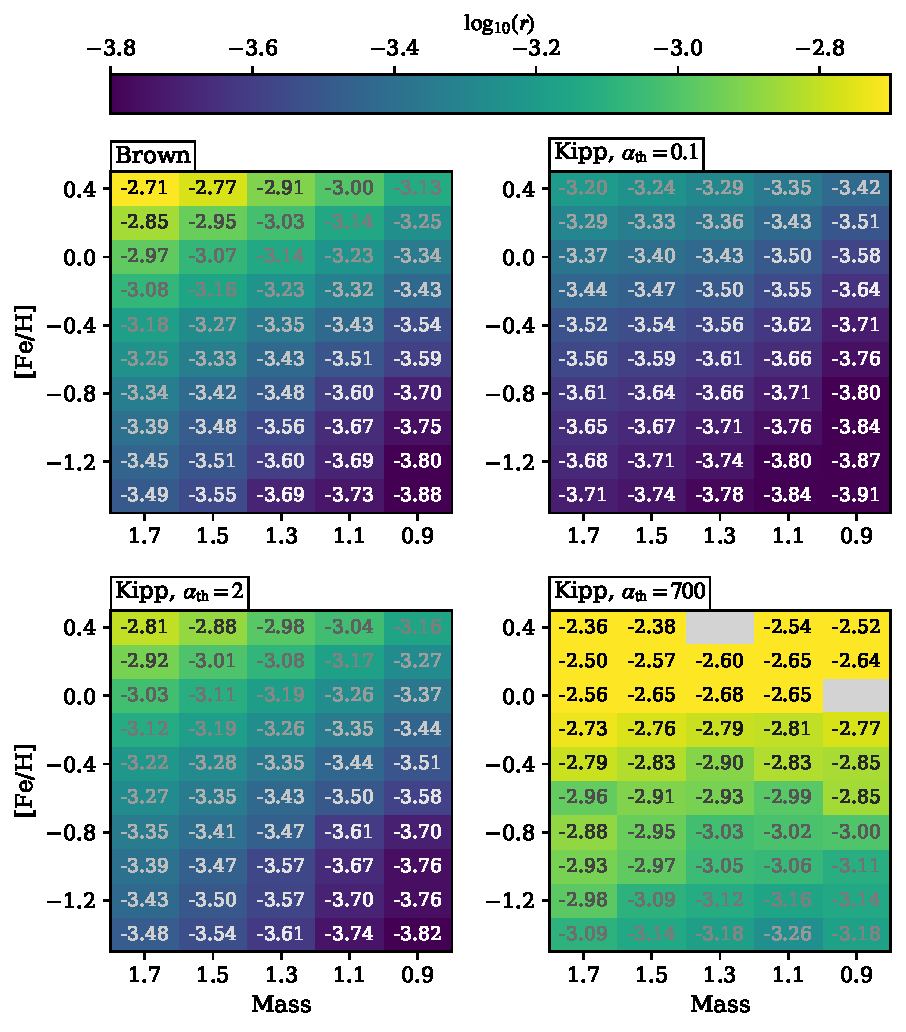
\includegraphics[width=\textwidth]{mesa_r_spread.pdf}
    \caption{The reduced density ratio $\log_{10} r$ is extracted as discussed in Section \ref{sec:mesa_experiment} for four grids of stellar models with differing prescriptions for thermohaline mixing. 
    Results for $\log_{10} r$ are shown as a function of stellar mass and metallicity [Fe/H], with high values of $\log_{10} r$ in brighter colors (yellow) and low values of $\log_{10} r$ in darker colors (purple). 
    The model name and mixing efficiency, $\alpha_{\text{th}}$ (where applicable) constitute the physical configuration and are indicated in the panel labels.}
    \label{fig:mesa_r_spread}
\end{figure*}